\documentclass[11pt,a4paper]{article}
\usepackage[latin1]{inputenc}
\usepackage[margin=1in]{geometry}
\usepackage{amsmath}
\usepackage{booktabs}
\usepackage{url}
\usepackage{amsfonts}
\usepackage{amssymb}
\usepackage{graphicx}
\usepackage{enumitem}
\setlength\abovedisplayskip{0pt}
\author{James Brissette}
\title{CS-6350: HW 4}
\begin{document}
	\maketitle
	
	\section{PAC Learning}
		\begin{itemize}
			\item [1.]
				\begin{enumerate} [label={\alph*)}]
					\item  Given N available parts, if we assume that two products made with parts $a$,$b$, and $c$ constitute the same hypothesis irrespective of the order in which the parts were used, then the total hypothesis space could be thought of in the following way:\\ 
					
					Suppose we had $N$ bins of products where the products in each bin were segregated by the number of parts they are made up of. In bin $1$, we have ${N \choose 1}$ or $N$ distinct products each consisting of one part, because there are $N$ total parts to choose from. In bin $2$ we would have ${N \choose 2}$ distinct products since that is how many ways we have to choose 2 products from a collection of size $N$. If we continued this we would follow the same pattern up to bucket $N$ where there is only $1$ way to choose all of the parts (assuming ordering doesn't matter).\\
					
					To summarize this mathematically, for a collection of $N$ available parts, we have 
					$${N \choose 1} + {N \choose 2} + \dots + {N \choose N} = \displaystyle\sum_{k=1}^{N} {N \choose k}$$
					\item Analyzing an experienced worker who follows both rules, we can take a similar approach, however, here we see that for bin $1$, the worker can now choose to use the whole part, or either of the distinct pieces. This changes our method of counting as follows:\\
					In bin $1$ the worker now has $N$ whole parts (as in part a), and also has an additional $2$ choices for each part if he decides to use the halves instead. This brings his total choices for each part to $3$ (whole part, first half, or second half). If he only chooses $1$ part, there are $3$ options; if he chooses $2$ parts, he has $3*3$ ways to combine them; and similarly if he chooses $k$ parts, he has $3_1*3_2*3_3* \dots = 3^k$ ways to assemble them. We see that since the worker can assemble $k$ parts $3^k$ different ways, and he has ${N \choose k}$ ways to choose $k$ parts, the total hypothesis space can be written as:
					
					$$\displaystyle\sum_{k=1}^{N} 3^k{N \choose k}$$
					
					\item From Occam's Razor we have $$m > \frac{1}{\epsilon} \Big( ln(\vert H \vert) + ln\frac{1}{\delta}\Big)$$
					Having calculated our hypothesis spaces in parts a and b, and knowing that the experienced worker is making the products (taking the hypothesis space from part b) we have that $H=\displaystyle\sum_{k=1}^{6} 3^k{6 \choose k}=4095$, and substituting in what we know yields the following:
					$$m > \frac{1}{.01} \Big( ln(\vert 4095 \vert) + ln\frac{1}{.01}\Big) > 1.292269e+03 $$
					for a total of at least 1293 examples.
					
				\end{enumerate}
				
			\item [2.]
				If we know that each concept in $C$ is a rectangle with integer valued boundaries, and we know that in a plane bounded by $(0,0)$ and $(n,n)$ that the number of said rectangles is $\Big( \frac{n(n+1)}{2} \Big)^2$, then we can use the fact that the integers $a,b,c,d$ are in the interval (0,20) to deduce that the total number of rectangle in that interval is $\Big( \frac{20(21)}{2} \Big)^2 = 44,100$. Using this result we calculate the upper bound is:
				$$m > \frac{1}{.01} \Big( ln(\vert 44100 \vert) + ln\frac{1}{.01}\Big) > 1.529939e+03 $$
				for a total of at least 1530 randomly drawn examples.
		\end{itemize}
		
	\section{Shattering}
		\begin{enumerate}
			\item I claim that the set of templates $H_n$ does not shatter the set $X_n$ for all values of $n$. To prove this we simply need to find one configuration of $X_n$ that is not shattered by $H_n$. First turning to the case where $n=1$ we see that there are for possible labelings of the set $X_1=\{0,1\}$:
			$$\begin{array}{c|c} 
				0  & 1  \\
				1  & 1  \\ 
				   &    \\
				0  &  1 \\
				1  & -1 \\
				   &    \\
				0  & -1 \\
				1  &  1 \\
				   &    \\
				0  & -1 \\
				1  & -1 \\
			\end{array}$$
			
			It is apparent in the first case that if the function $h_1 = \{-\}$ where $h_1 \in H_1 = \{1,0,-\}$ that the function matches to both points and correctly labels them. Likewise in the second case we reach into our bag and pull out $h_1 = \{0\}$. Here we find that $0$ is matched and returns a $1$ as expected, and $1$ doesn't match, returning a $-1$. The same can be found in the third case when $h_1=\{ 1\}$.\\
			
			However, what we find is that in the last case where both labelings are $-1$ that we see this fails. In this case there is no function in $H_1$ that doesn't match to \textit{at least} 0 or 1. Because there exists a labeling in $n=1$ in which $h_1$ is not expressive enough to correctly match all possible labelings we cannot say that $H_n$ shatters $X_n$ for $n=1$
			
			We can extend this to the general case arbitrary $n$ by recognizing that for any value of $n$ there exists at LEAST one labeling for each element in $X_n$ in which every element is labeled with $=-1$. We can see that there is $H_n$ does not contain a function of length $n$ in which it does not match to both a $1$ and a $0$ simultaneously. Thus for $n=2$, our counter-example is $$\begin{array}{c|c} 
				00  & -1 \\
				01  & -1 \\
				10  & -1 \\
				11  & -1
			\end{array}$$
			and similarly for $n=3,4,\dots,\infty$
		\end{enumerate}
	
	\section{VC Dimensions}
		\begin{itemize}
			\item [1.]
				\begin{enumerate} [label={\alph*)}]
					\item  The VC dimension for the concept class $H_c$ consisting of circles depends on our definition of circles. If we define circles to be "perfect", as in all points along the circles boundaries are equidistant from the center, then the VC dimension is 3. First, we see that perfect circle are expressive enough to shatter one and two points trivially:
					\begin{center}
						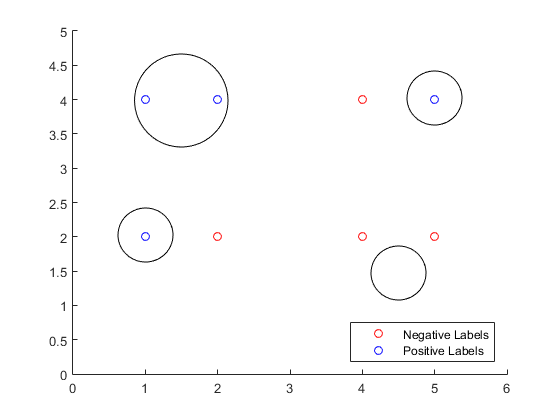
\includegraphics[width=1\linewidth]{q3a}
					\end{center}
					
					With three points, we start to see some challenges. There are two primary configurations of three points: three colinear points, and three points forming a triangle. Here we see that for the colinear points, there exists a configuration that is not separable, but for the triangle, all labelings are separable:
					\begin{center}
						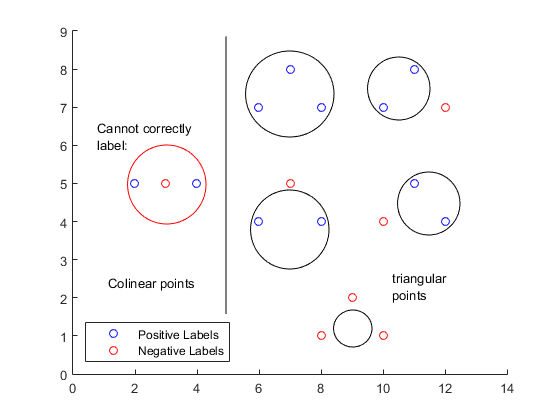
\includegraphics[width=.75\linewidth]{q3a_2}
					\end{center}
					
					Now if we are assuming perfect circle, there does not exist a configuration of four points in which ALL of the labelings are correctly classifiable using circles. Since we've shown three colinear points is not shattered by circles, we know there is at least one labeling that can't be correctly seperated if we our four-point configuration included three colinear points. So what's left to try is three points in a triangle with the fourth point located inside the shape, or four points forming two distinct triangles. Noteworthy in this is that neither layout is separable using perfect circles. The left example is clear, but on the right, we see that it is not possible to touch opposite corners without touching all four points:
					\begin{center}
						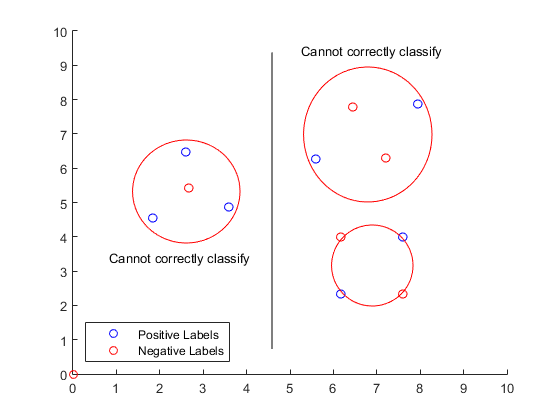
\includegraphics[width=.75\linewidth]{q3a_4}
					\end{center}
									
					If, however, we relax our assumptions of circles to include shapes such as ellipses then we could argue the VC dimension further by overcoming the limitation that we can't touch opposite corners without touching all four points. In this case we've already proved that you can shatter 2 points, and every pair of 4 points could be reached independent of the other two.
					
					\item For this concept class, we see that for any \textit{individual} point, we can correctly classify the labeling by moving the shaded region given by $x_1 \geq a$, $x_2 \leq b$ on or off the point. However given that this concept class labels everything below and to the right of the point($x_1,x_2$) as positive, we see there is only one configuration of two points that is correctly classifiable, where the slope of the line connecting the two points is positive (e.g. the points are diagonal with one being above and to the right of the other):
					\begin{center}
						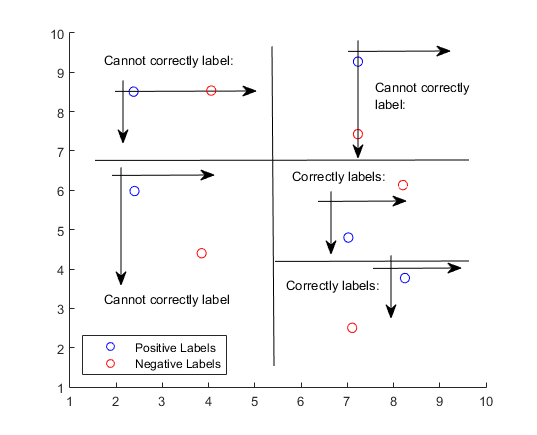
\includegraphics[width=1\linewidth]{q3b}
					\end{center}
					
					We see this hypothesis class does not shatter two points because it fails to correctly classify them when they are arranged vertically, horizontally, or along a line with a negative slope. However, because it does shatter two points for all labelings where the points are placed along a line with a positive slope, the VC dimension is $\geq 2$.\\
					
					Unfortunately we see with three or more points, that this is no longer the case. We've seen that vertical and horizontally aligned points and points along a line with a negative slope fail to be classified correctly, and three points or more points can be generalized as a groups of two points arranged in the same pattern. If any of the two points are aligned in one of the three ways mentioned above, we will be able to find a way to label them such that the concept class can not shatter it. The last case is if they are all colinear and along a line with a positive slope, but in the following plot, we see a labeling that fails to correctly classify, thus the VC dimension is 2:
					\begin{center}
						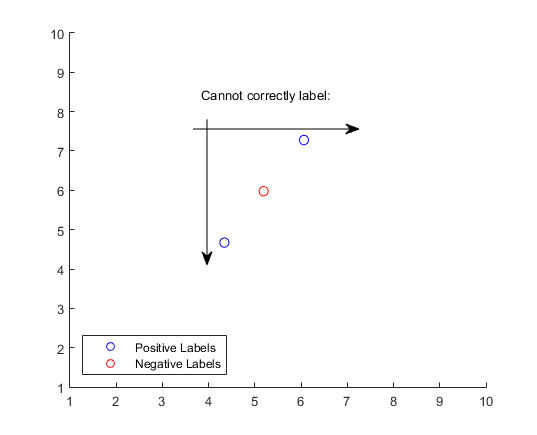
\includegraphics[width=1\linewidth]{q3b_2}
					\end{center}
					
				\end{enumerate}
				
			\item [2.]
				We know that the VC dimension of a hypothesis space $H$ measures the complexity of $H$ by counting the number of instances of $X$ that can be shattered, and while it does not strictly depend on the size of the hypothesis class, we see that if we were to start taking subsets $H_2$ of $H_1$, or in other words if we were to take $H_2 \subseteq H_1$, then it follows that $\vert H_2 \vert \leq \vert H_1 \vert$. If at \textit{any} point our subset does not contain the most expressive hypotheses from the class $H_1$, then the VC dimension of our subset $H_2$ will be less than then our complete hypothesis space $H_1$.\\
				
				We also know from Vapnik that the VC dimension of $H$ is bounded by the dimensionality $D$ of the data points in X and the radius/margin of the data set (e.g min $\Big[ D,$ ceiling($\frac{4R^2}{\gamma^2}) \Big]$). From this we see the smaller the radius or the larger the margin becomes, the smaller the VC dimension becomes, which is certainly the case as we start taking subsets.\\
				
				Alternatively, if our subset is finite, we know the VC dimension is $\leq log_2 \vert H \vert$ and if we take $H_2 \subseteq H_1$, then $\vert H_2 \vert \leq \vert H_1 \vert$.
				
				Lastly, if $VC(H_2) = d$ and we know that $H_2 \subseteq H_1$ then we know that the size of $H_1$ is no smaller than $H_2$, meaning the same functions exist and that $VC(H_1) \geq VC(H_2)$. What we now consider is the possibility that $H_1$ contains additional more \textit{expressive} functions than $H_2$. With this it is certainly possible that we will eventually stumble upon a space in which the functions are expressive enough to increase the VC dimension of $H_1$.
		\end{itemize}
	
	\section{AdaBoost}
		\begin{itemize}
			\item [1.]
			At the end of round 1 we compute $\epsilon_1$ as $$\displaystyle\sum_{i} D_t (i) \quad where \quad y_i \neq h(x_i) \rightarrow \epsilon_1 = \frac{1}{4} $$ We then use $\epsilon_1$ to solve for $\alpha_1$ as $$\alpha_1 = \frac{1}{2} ln \Big( \frac{1-\epsilon_1}{\epsilon_1} \Big) = 0.5493$$. We then calculate $D_2$ using $$D_2(i) = \frac{D_1(i)}{Z_t}*e^{-\alpha_t y_i h_1(x_i)}$$ Results are as follows:\\
			
				\textbf{Round 1:}
				\begin{center}
					\begin{tabular}{rccccc}
						\toprule
						${\bf x} = [x_1,x_2]$ & $y_i$ & $f_a(x)$ & $D_1$ & $D_{1}(i)y_{i}h_t({\bf x_i})$ & $D_2$ \\
						\midrule
						$[1,  1]$             & -1    & 1        & 1/4   & -1/4                          &  .5000     \\
						$[1, -1]$             & 1     & 1        & 1/4   & 1/4                           &  .1667     \\
						$[-1,-1]$             & -1    & -1       & 1/4   & 1/4                           &  .1667     \\
						$[-1, 1]$             & -1    & -1       & 1/4   & 1/4                           &  .1667     \\
						\bottomrule
					\end{tabular}
				\end{center}
			$\epsilon_1 = 1/4, \alpha_1 = \frac{\ln3}{2}, Z_1 = \frac{\sqrt{3}}{2}$ \\
			
			For round 2 we will choose $h_2(x) = f_d(x) = -sgn(x_2)$. At the end of round 2 we compute $\epsilon_2$ as $$\displaystyle\sum_{i} D_t (i) \quad where \quad y_i \neq h(x_i) \rightarrow \epsilon_2 = 0.1667 $$ We then use $\epsilon_2$ to solve for $\alpha_2$ as $$\alpha_2 = \frac{1}{2} ln \Big( \frac{1-\epsilon_2}{\epsilon_2} \Big) = 0.8047$$. We then calculate $Z_2$ as $$Z_2 = \displaystyle\sum_{i=1}^4 D_t(i)*exp[-\alpha_t y_i h_2(x_i)] = 0.7454$$
			
			And lastly we calculate $D_3$ using $$D_3(i) = \frac{D_2(i)}{Z_2}*e^{-\alpha_2 y_i h_2(x_i)}$$ Results are as follows:\\
			
			\textbf{Round 2:}
			\begin{center}
				\begin{tabular}{rccccc}
					\toprule
					${\bf x} = [x_1,x_2]$ & $y_i$ & $f_d(x)$ & $D_2$ & $D_{2}(i)y_{i}h_t({\bf x_i})$ & $D_3$ \\
					\midrule
					$[1,  1]$             & -1    & -1       & .5000   & .5000                       &  .3000     \\
					$[1, -1]$             & 1     & 1        & .1667   & .1667                       &  .1000     \\
					$[-1,-1]$             & -1    & 1        & .1667   & -.1667                      &  .5000     \\
					$[-1, 1]$             & -1    & -1       & .1667   & .1667                       &  .1000     \\
					\bottomrule
				\end{tabular}
			\end{center}
			$\epsilon_2 = 0.1667, \alpha_2 = 0.8047, Z_2 = 0.7454$ \\
			
			For round 3 we will choose $h_3(x) = f_b(x) = sgn(x_1 - 2)$. At the end of round 3 we compute $\epsilon_3$ as $$\displaystyle\sum_{i} D_t (i) \quad where \quad y_i \neq h(x_i) \rightarrow \epsilon_3 = 0.1000 $$ We then use $\epsilon_3$ to solve for $\alpha_3$ as $$\alpha_3 = \frac{1}{2} ln \Big( \frac{1-\epsilon_3}{\epsilon_3} \Big) = 1.0986$$. We then calculate $Z_3$ as $$Z_3 = \displaystyle\sum_{i=1}^4 D_t(i)*exp[-\alpha_t y_i h_3(x_i)] = 0.6000$$
			
			And lastly we calculate $D_4$ using $$D_4(i) = \frac{D_3(i)}{Z_3}*e^{-\alpha_3 y_i h_3(x_i)}$$ Results are as follows:\\
			
			\textbf{Round 3:}
			\begin{center}
				\begin{tabular}{rccccc}
					\toprule
					${\bf x} = [x_1,x_2]$ & $y_i$ & $f_d(x)$ & $D_3$ & $D_{3}(i)y_{i}h_t({\bf x_i})$ & $D_4$ \\
					\midrule
					$[1,  1]$             & -1    & -1       & .3000   & .3000                       & .1667      \\
					$[1, -1]$             & 1     & -1       & .1000   & -.1000                      & .5000      \\
					$[-1,-1]$             & -1    & -1       & .5000   & .5000                       & .2778      \\
					$[-1, 1]$             & -1    & -1       & .1000   & .1000                       & .0556      \\
					\bottomrule
				\end{tabular}
			\end{center}
			$\epsilon_3 = 0.1000, \alpha_3 = 1.0986, Z_3 = 0.6000$ \\
			
			For round 4 we would like to choose $h_4(x) = f_c(x) = -sgn(x_1)$ since that weak classifier hasn't been utilized yet but we see that if we do it will incorrectly predict $x_2$ and give us an error $\geq \frac{1}{2}$. Instead we will use $h_4(x) = f_a(x) = sgn(x_1)$.  At the end of round 4 we compute $\epsilon_4$ as $$\displaystyle\sum_{i} D_t (i) \quad where \quad y_i \neq h(x_i) \rightarrow \epsilon_4 = 0.1667$$ We then use $\epsilon_4$ to solve for $\alpha_4$ as $$\alpha_4 = \frac{1}{2} ln \Big( \frac{1-\epsilon_4}{\epsilon_4} \Big) = 0.8047$$. We then calculate $Z_4$ as $$Z_4 = \displaystyle\sum_{i=1}^4 D_t(i)*exp[-\alpha_t y_i h_4(x_i)] = 0.7454$$
			
			And lastly we calculate $D_5$ using $$D_5(i) = \frac{D_4(i)}{Z_4}*e^{-\alpha_4 y_i h_4(x_i)}$$ Results are as follows:\\
			
			\textbf{Round 4:}
			\begin{center}
				\begin{tabular}{rccccc}
					\toprule
					${\bf x} = [x_1,x_2]$ & $y_i$ & $f_a(x)$ & $D_4$ & $D_{4}(i)y_{i}h_t({\bf x_i})$ & $D_5$ \\
					\midrule
					$[1,  1]$             & -1    & 1        & .1667 & -.1667                        & .5000      \\
					$[1, -1]$             & 1     & 1        & .5000 & .5000                         & .3000      \\
					$[-1,-1]$             & -1    & -1       & .2778 & .2778                         & .1667      \\
					$[-1, 1]$             & -1    & -1       & .0556 & .0556                         & .0333      \\
					\bottomrule
				\end{tabular}
			\end{center}
			$\epsilon_4 = 0.1667, \alpha_4 = 0.8047, Z_4 = 0.7454$ \\
			
			At this point we have a total of 4 rounds and we compute our final hypothesis $H_{final}$ as
			\begin{align*}
				H_{final} &= sgn \Big[ \alpha_1 h_1 + \alpha_2 h_2 + \alpha_3 h_3 + \alpha_4 h_4 \Big] \\
				 &= sgn \Big[ .5493*sgn(x_1) + .8047 *-sgn(x_2) + 1.0986 *sgn(x_1 - 2) + .8047*sgn(x_1) \Big]
			\end{align*}
		\end{itemize}
	
\end{document}